\section{Verwandte Arbeiten}

\subsection{Arbeit 1}
\textcite{bazurto2019} beschäftigen sich mit sehr ähnliche Problemstellungen zu dieser Arbeit in Bezug auf den World Happiness Report. Sie stellen einen Mangel an Interaktivität und intuitiver Erforschung der Berichtdaten fest. Auch vergleichen sie dessen Visualisierungen mit denen des OECD Happiness Reports. Für diese Arbeit sind allerdings nur die Teile mit Bezug auf den World Happiness Report von Bedeutung. 

Sie setzen sich 6 Zielen, welche sie mittels Interaktiver Visualisierungen erreichen wollen. Diese Ziele Lauten:

\begin{itemize}
\item 1. Present the ranking, countries and their respective score

\item 2. Discover happiness distribution in the world. The user can interact with each country to obtain details on demand.
\item 3. Identify the happiness score and indexes by country

\item 4. Locate (knowing the country that I want to find (e.g. my country) a country and query how happy is it and how indexes are in this.

\item 5. Identify which countries are happier and which ones less happy extremes

\item 6. Discover happiness distribution in the different world regions. The user can interact with each country in those regions to obtain details on demand.
\end{itemize}

Hier ist viel Überschneidung mit den Zielen und Visualisierungen dieses Berichtes zu finden. Für die meisten dieser Ziele bietet auch dieser Bericht eine Antwort. Punkt 2,5 und 6 lassen sich durch den Scatterplot abdecken und 3 sowie 4 lassen sich durch eine Suche im Polarplot Dropdown beantworten. \\

Die Autoren entscheiden sich für insgesamt 5 Visualisierungen welche im Zusammenspiel diese Fragen beantworten sollen. Diese sind: Choroplethenkarte, Parallel Plot, Bar Chart, Ranking List sowie ein Bubble Chart. 
Die beste Vergleichsgrundlage bildet wohl Abbildung.\ref{fig:bazurto} , hier sind 
Die Choroplethenkarte, der Parallelplot und das Ranking enhalten. 
Wie bereits in der Schilderung der Visualisierungen erwähnt wäre der Parallelplot eine Alternative zum Polarplot gewesen. Hier ist der Unterschied deutlich zu sehen.
Es ist nun möglich die Dimensionen für alle Länder gleichzeitig darzustellen. Die Authoren haben hier das Problem der Sichtbarkeit gut gelöst, indem sie das ausgewählte Land Farblich hervorheben und die anderen Linien nur durch ein leichtes grau einzeichnen. Die anderen Linien tragen hier dennoch nicht viel Informationen bei, es lassen sich hier nicht wirklich zusätzliche Muster aus den Daten lesen das die Linen ineinander verschwinden.\\

Wirklich interessant und auch sehr intuitiv wirkt die Chloroplethenkarte. Hier lässt sich ein guter Überblick Über den Happiness-Score in der ganzen Welt gewinnen. Der Scatterplot ist nicht in der Lage die geographische Gruppierung so gut abzubilden wie eine Karte. Die Sublementierung mit der Regionenlegende ist nicht so Aussagekräftig. 

\cite{bazurto2019}
\begin{figure}[h]
 \centering
 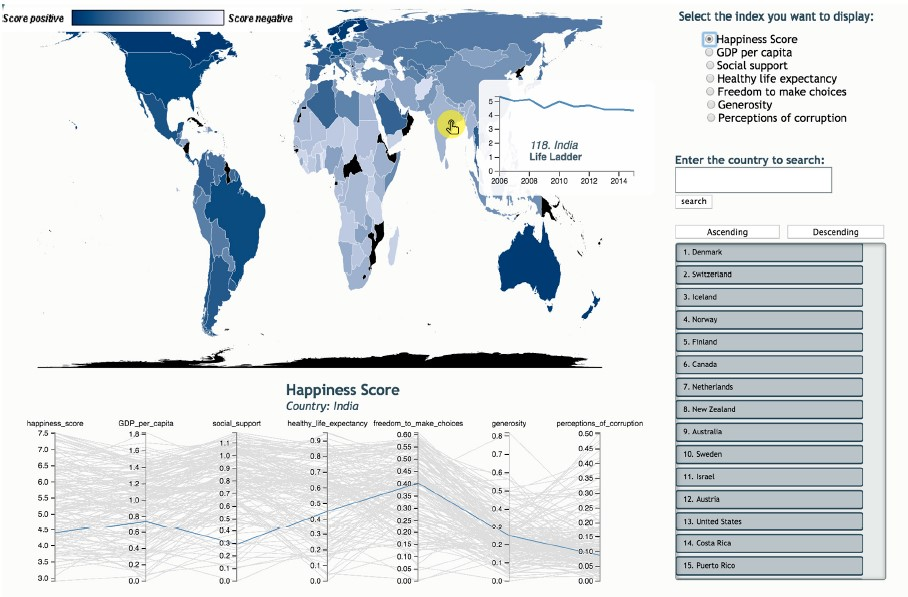
\includegraphics[width = 0.8\textwidth]{img/bazurto_vis.jpg}
 \caption{Visualisierung aus \textcite{bazurto2019}}
 \label{fig:bazurto}
\end{figure}

\subsection{Arbeit 2}